% arara: pdflatex
% arara: biber if (missing("bbl") || changed("bib"))
% arara: pdflatex if (missing("bbl") || changed("bbl"))
% arara: pdflatex if (found("log", "Label(s) may have changed."))
\documentclass[portuguese]{beamer}
\usepackage[version=3]{mhchem}

\usepackage[utf8]{inputenc}
\usepackage[T1]{fontenc}
\usepackage{babel}
\usepackage{microtype}
\usepackage{xcolor}
\usepackage{anyfontsize}
\usepackage{pdflscape}
\usepackage{bbding}

% -- Tipo de letra
\usepackage{mathpazo}
%\usepackage{newpxtext}
%\usepackage{eulervm}
\usepackage{nimbusmono}

% -- Funções matemáticas extra
\usepackage{mathtools}
\usepackage{siunitx}

% -- Símbolos extra
\usepackage{amssymb}

\usepackage{textcomp}
\usepackage{gensymb}
\usepackage{cancel}

% -- Bibliografia
\usepackage[
	backend = biber,
	style = numeric,
	sorting = ynt
	]{biblatex}
\usepackage{fvextra}
\usepackage{csquotes}

% --  Definições de imagens
\usepackage{graphicx}
\graphicspath{{graphics/}}
\usepackage{caption}
\usepackage{subcaption}
\usepackage{afterpage}
\usepackage{tabularx}
%\usepackage[labelformat=empty]{caption}
\usepackage{multicol}
\usepackage{multirow}
\usepackage{booktabs}
\usepackage[export]{adjustbox}
\usepackage{caption}

% -- Desenhar circuitos elétricos e lógicos
\usepackage{tikz}
\usepackage{pgfplots}
\usetikzlibrary{arrows.meta,positioning}
\pgfplotsset{compat=1.5}
\pgfplotsset{table/search path = {data}}
\pgfplotsset{	/pgf/number format/use comma,}


\usepackage{todonotes}

%%%%%%%%%%%%%%%%%%%%%%%%%%%%%%
%Cenas do beamer

\addbibresource{../report/main.bib}
\addbibresource{main.bib}
\definecolor{istblue}{RGB}{0,157,224} % ist blue)

% símbolo de "certinho"
\def\checkmark{\tikz\fill[scale=0.4](0,.35) -- (.25,0) -- (1,.7) -- (.25,.15) -- cycle;} 
\mode<presentation>
{
  \usetheme{Madrid}       % or try default, Darmstadt, Warsaw, ...
  \usecolortheme{orchid} % or try albatross, beaver, crane, ...
  \usecolortheme[named=istblue]{structure}
  \usefonttheme{serif}    % or try default, structurebold, ...
  \setbeamertemplate{navigation symbols}{}
  \setbeamertemplate{caption}[numbered]
  \setbeamertemplate{itemize items}[circle] %ball,circle, square
  
} 

\setbeamertemplate{bibliography item}{\insertbiblabel}
\setbeamertemplate{caption}{\raggedright\insertcaption\par}

\setbeamertemplate{caption}[numbered]
\setbeamerfont{institute}{size=\Large}
\setbeamerfont{date}{size=\small}
\setbeamerfont{author}{size=\small}




\title[Radar MIMO]{Radar MIMO}


\author[MEAer -- Sistemas de Radar]{
  João Gonçalves 81040 \and Daniel de Schiffart 81479
    }

\institute{Sistemas de Radar}
\date{Dezembro de 2018}
\setbeamertemplate{footline}
{
  \leavevmode%
  \hbox{%
  \begin{beamercolorbox}[wd=.333333\paperwidth,ht=2.25ex,dp=1ex,center]{author in head/foot}%
    \usebeamerfont{author in head/foot}\insertshortauthor
  \end{beamercolorbox}%
  \begin{beamercolorbox}[wd=.333333\paperwidth,ht=2.25ex,dp=1ex,center]{title in head/foot}%
    \usebeamerfont{title in head/foot}\insertshorttitle
  \end{beamercolorbox}%
  \begin{beamercolorbox}[wd=.333333\paperwidth,ht=2.25ex,dp=1ex,right]{date in head/foot}%
    \usebeamerfont{date in head/foot}Trabalho de síntese\hspace*{2em}
    \insertframenumber{} / \inserttotalframenumber\hspace*{2ex} 
  \end{beamercolorbox}}%
  \vskip0pt%
}

%%%%%%%%%%%%%%%%%%%%%%%%%%%%%%%%%%%%%%%%%%%%%%%%%%%%%%%%%%%%%%
\begin{document}

\begin{frame}
    \begin{figure}
	
\includegraphics[width=0.5\linewidth]{graphics/tecnico_logo.png}
    \end{figure}
    \titlepage
\end{frame}
\setbeamertemplate{section in toc}[circle]
\begin{frame}{Conteúdo}
  \tableofcontents
\end{frame}

\section{Conceito MIMO}

\begin{frame}{Conceito MIMO}
  \begin{figure}[]
	\centering
	\begin{minipage}[t]{0.5\linewidth}
	  \centering
	  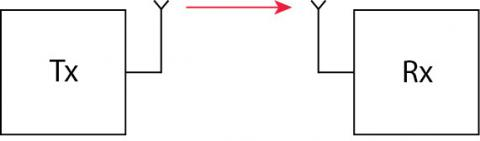
\includegraphics[width=0.7\linewidth]{com1.jpg}
    \end{minipage}%
    \begin{minipage}[t]{0.5\linewidth}	
	  \centering
	  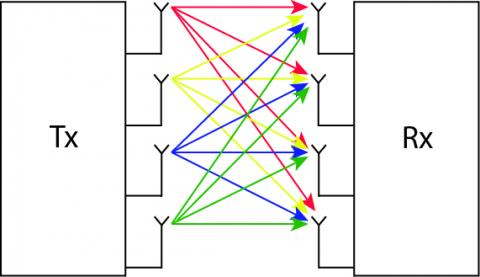
\includegraphics[width=0.7\linewidth]{com2.jpg}
    \end{minipage}%
	\caption{Sistema SISO e MIMO. Fonte: \cite{swantennas}.}
	\label{fig:antenas}
  \end{figure}
  Vantagens
  \begin{itemize}
	\item Explora a diversidade espacial.
	\item \textit{Streams} de informação redundante.
  \end{itemize}
\end{frame}

\begin{frame}{Radar MIMO}
  \par
  {\large Radar MIMO -- \textit{multi-input multi-output}} 
  \begin{itemize}
	\item Generalização do radar multiestático.
  \end{itemize}
  \begin{figure}[]
	\centering
	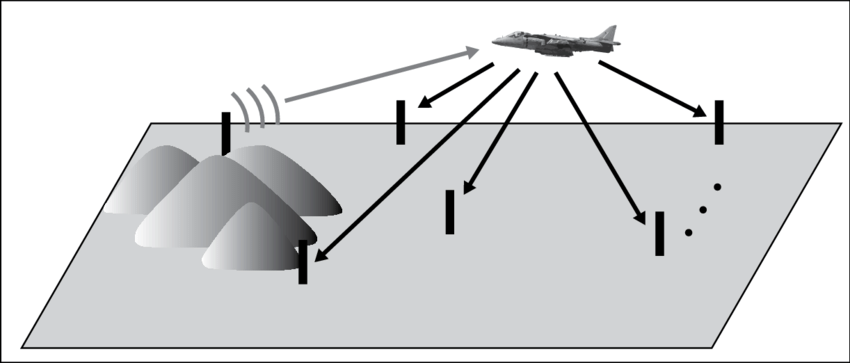
\includegraphics[width=0.8\linewidth]{../report/graphics/multistatic.png}
	\caption{Radar multiestático. Fonte: \cite{mimoradarbook}}
	\label{fig:mono}
  \end{figure}
\end{frame}

\section{Radar MIMO}

\begin{frame}{Radar MIMO}
  \begin{itemize}
	\item Radar MIMO coerente -- generalização do mono-estático.
  \end{itemize}
  \begin{figure}[]
	\centering
	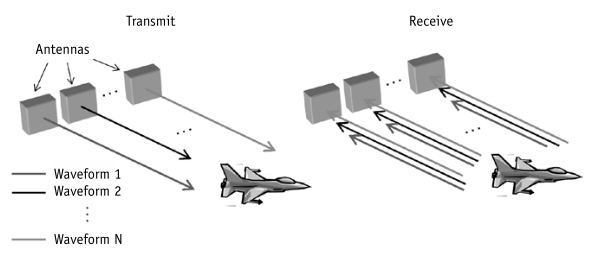
\includegraphics[width=0.7\linewidth]{../report/graphics/concept.png}
	\caption{Radar MIMO coerente. Fonte: \cite{mimoradarbook}.}
	\label{fig:concept}
  \end{figure}
\end{frame}

\begin{frame}{Agregado virtual}
  Com formas de onda ortogonais, pode-se analizar um radar MIMO coerente como um agregado virtual.
  \begin{align*}
    \left\{ \frac{x_{Tm}+x_{Rn}}{2}:\; m=1,\ldots,M;\,n=1,\ldots,N \right\}
  \end{align*}
\end{frame}

\begin{frame}{Agregado virtual}
  \begin{figure}[]
	\centering
	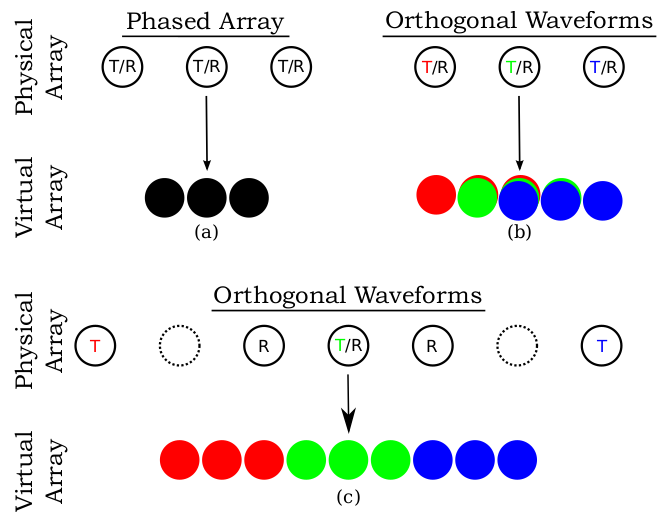
\includegraphics[height=5.5cm]{../report/graphics/virt1.png}
	\caption{Agregado virtual MIMO. Fonte: \cite{davis2015mimo}.}
	\label{fig:virt1}
  \end{figure}
\end{frame}

\section{Processamento de Sinais}

\begin{frame}{Processamento de Sinais}
  \begin{figure}[]
	\centering
	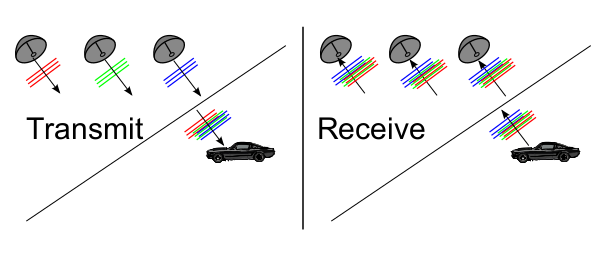
\includegraphics[width=0.9\linewidth]{../report/graphics/rad3.png}
	\caption{MIMO com $M=N=3$. Fonte: \cite{davis2015mimo}.}
	\label{fig:r3}
  \end{figure}
  \begin{align*}
    \mathbf{y}(t,\theta_0) = \alpha\mathbf{b}(\theta_0)\mathbf{a}(\theta_0)^T\mathbf{x}(t)+\mathbf{v}(t)
  \end{align*}
\end{frame}

\begin{frame}{Processamento de Sinais}
  \begin{figure}[]
	\centering
	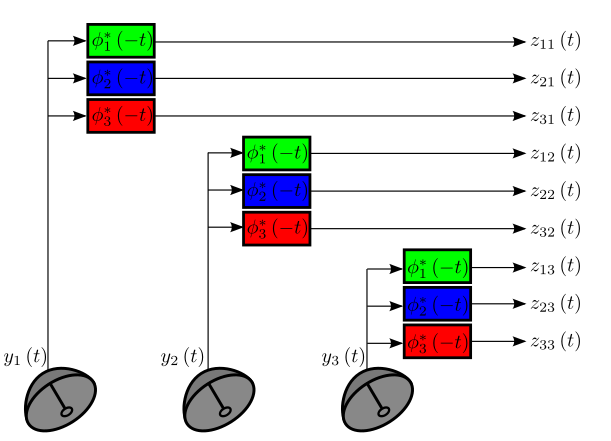
\includegraphics[height=6.5cm]{../report/graphics/processor.png}
	\caption{Separação dos sinais observados. Fonte: \cite{davis2015mimo}.}
	\label{fig:proc}
  \end{figure}
\end{frame}

\begin{frame}{Processamento de Sinais}
  \par
  \small
  \begin{align*}
    p_d &= exp\left( -\frac{\gamma}{\sigma_t^2 + \sigma_n^2} \right)  \\
    p_{fa} &= exp\left( -\frac{\gamma}{\sigma_n^2} \right) 
  \end{align*}
  \begin{figure}[]
	\centering
	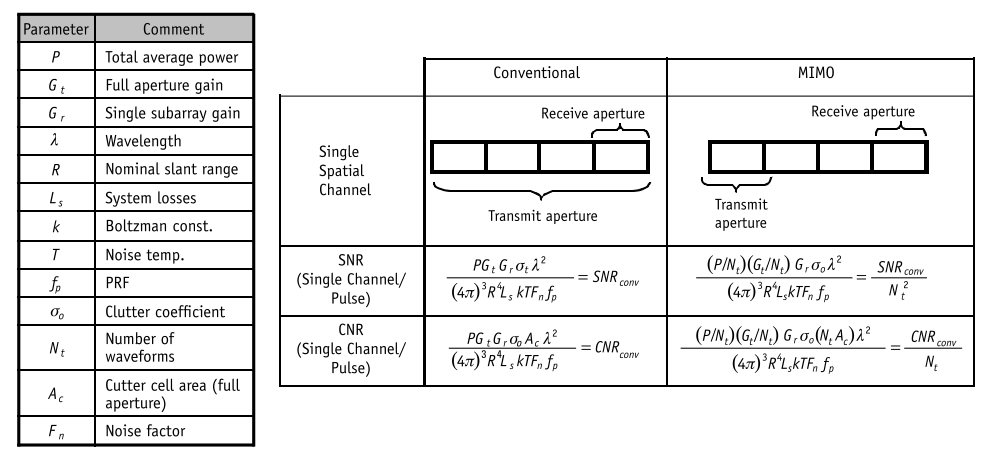
\includegraphics[width=0.9\linewidth]{../report/graphics/table.png}
	\caption{Sensibilidade de MIMO coerente. Fonte: \ref{mimoradarbook}.}
	\label{fig:tabela}
  \end{figure}
\end{frame}

\section{Aplicações}

\begin{frame}{Imagens de Radar}
	\begin{figure}[ht]
		\centering
		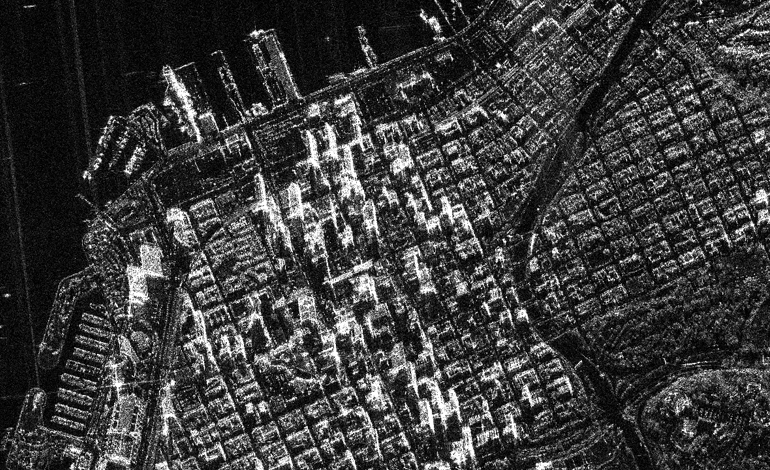
\includegraphics[width = 0.7\textwidth]{../report/graphics/sandiego.jpg}
%		\caption{Exemplo de imagem obtida por radar, através de SAR.}
		\label{fig:sandiego}
	\end{figure}
\end{frame}

\begin{frame}{Radar de Abertura Sintética - SAR}
	\begin{figure}
		\centering
		\begin{minipage}[t]{0.43\textwidth}
			\centering
			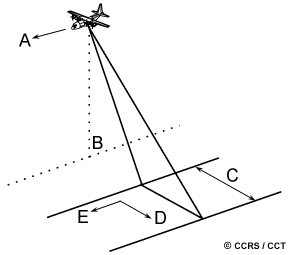
\includegraphics[height=3.3cm]{../report/graphics/radgeom.png}
%			\subcaption{Esquema geral do uso de SAR. Na imagem os rótulos representam \figlabel{A} a trajetória de voo, \figlabel{B} o \textit{nadir}, \figlabel{C} a faixa iluminada a cada instante, \figlabel{D} o alcance a cada instante e \figlabel{E} a zona iluminada prevista na trajetória.}
			\label{subfig:sar-side}
		\end{minipage}
		\hfill
		\begin{minipage}[t]{0.43\textwidth}
			\centering
			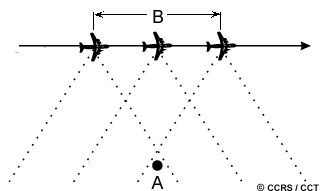
\includegraphics[height=3.3cm]{../report/graphics/sar.png}
%			\subcaption{Captação de imagens em movimento são utilizadas como perspetivas diferentes. Quando um alvo \textbf{A} entra no alcance do radar, inicia-se o cálculo da distância entre antenas simuladas \textbf{B}, que é o segmento máximo da trajetória em que \textbf{A} se encontra em alcance.}
			\label{subfig:sar-timesteps}
		\end{minipage}
		\caption{Radar de Abertura Sintética.}
		\label{fig:nrcan}
	\end{figure}
	\begin{align*}
		\delta_x &\triangleq \frac{v}{f_p}
		& ACR &\triangleq vR_{\textrm{swath}} \\
		R_{\textrm{swath}} &< \frac{c/2}{f_p}
		& ACR &< \delta_x\left(\frac{c}{2}\right)
	\end{align*}
\end{frame}

\begin{frame}{Radar Automóvel}
	\begin{figure}
		\centering
		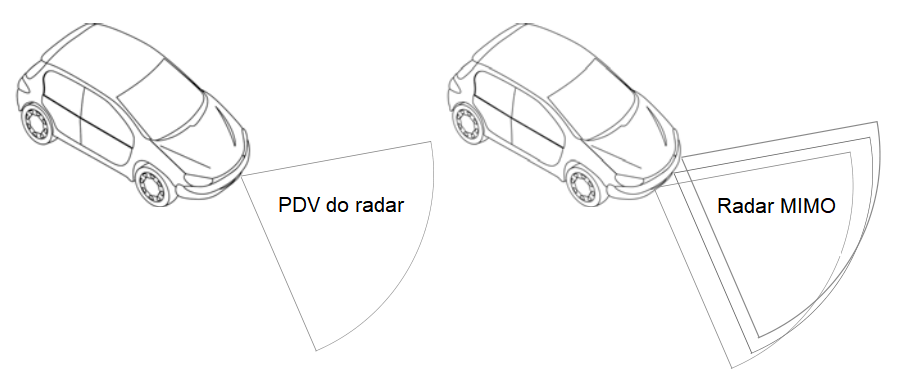
\includegraphics[width=0.7\textwidth]{../report/graphics/auto.png}
		\caption{Radar automóvel dianteiro.}
		\label{fig:autorad}
	\end{figure}
\end{frame}

\begin{frame}{Radar Além-Horizonte}
	\begin{figure}
		\centering
		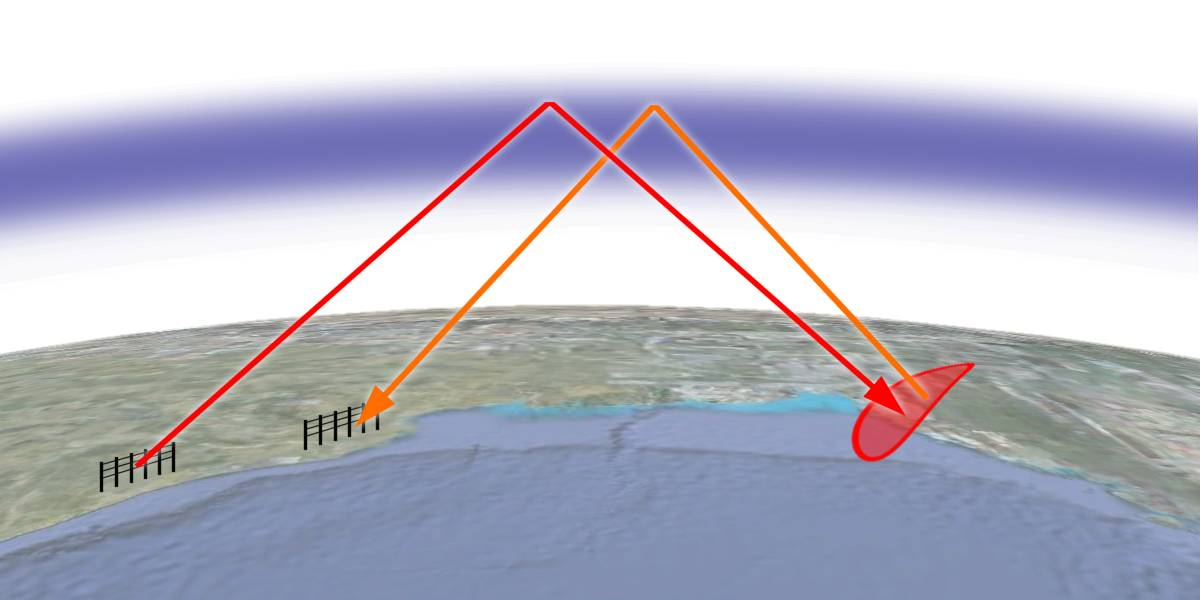
\includegraphics[width=0.7\textwidth]{oth-b.jpg}
		\caption{Radar Além-Horizonte, ou OTH (\textit{Over The Horizon}).}
		\label{fig:oth-b}
	\end{figure}
\end{frame}

\begin{frame}{Radar Além-Horizonte}
	\begin{figure}[ht]
		\centering
		\begin{tikzpicture}[]
			\path [pattern = crosshatch dots, pattern color = white!80!black,draw=white!70!black] (1,0) -- ++(1,0) arc (0:33.69:1) -- cycle;
			\node at (2.2,0.3) [] {$\phi$};
			\path [draw=white!40!black,thick] (0,0) -- (8,0);
			\path [draw=white!60!black,thick] (0,2) -- (8,2);
			\path [draw=white!80!black,thick] (0,4) -- (8,4);
			\node (radar) at (1,0) [circle,fill,inner sep = 1pt,label={135:Radar}] {};
			\path [draw,-{Latex[round]},dashed] (radar) -> (4,2);
			\path [draw,-{Latex[round]},dashed] (4,2) -> (7,0);
			\path [draw,-{Latex[round]},dashed] (radar) -> (4,4);
			\path [draw,-{Latex[round]},dashed] (4,4) -> (7,0);
			\node (target) at (7,0) [circle,fill,inner sep = 1pt,label={45:Alvo}] {};
		\end{tikzpicture}
		\caption{Exemplificação das reflexões atmosféricas e múltiplos trajetos para o alvo com radar OTH.}
		\label{fig:oth}
	\end{figure}
\end{frame}

\section{Dificuldades}

\begin{frame}{Dificuldades}
  A implementação do radar MIMO traz alguns problemas práticos
  \vspace{10pt}
  \begin{itemize}
    \item Complexidade de computação
	\item Rejeição adaptativa de clutter
	\item Problemas de calibração e equalização
	\item Constrangimentos de Hardware
  \end{itemize}
\end{frame}

\begin{frame}{Computação}
  Em processamento digital, as tarefas mais complexas são:
  \begin{itemize}
	\item Compressão de pulsos
	\item Processamento Doppler
	\item Rejeição de clutter
  \end{itemize}
  Fração de FLOPS:
  \begin{align*}
	f_{pre} &= 1+ \frac{\log_2 N}{\log_2 (LM)}\, &&\longrightarrow \textrm{convolução com FFTs}
 \\
	f_c &= M\left( \frac{MN^3+L}{M^2N^2+L} \right) \, &&\longrightarrow \textrm{Algoritmos STAP}
  \end{align*}
\end{frame}

\section{Conclusão}

\begin{frame}{Conclusões}
  Radar MIMO pode melhorar os sistemas convencionais nos ramos de
  \begin{itemize}
	\item Imagens por Radar
	\item Radar \textit{Over-the-Horizon} 
	\item \textit{Airborne surface surveillance}
  \end{itemize}
  Em muitos outros sistemas não oferece melhorias.

  \vspace{20pt}

  Tecnologia recente e em desenvolvimento.
  \begin{itemize}
	\item Primeira aparência nos anos 90
	\item Abundância de artigos sobre radar MIMO nos últimos 15 anos
  \end{itemize}

\end{frame}

\begin{frame}{Referências}
  \printbibliography
\end{frame}

\end{document}

